% Created 2021-08-17 Tue 20:22
% Intended LaTeX compiler: pdflatex
\documentclass[11pt,twoside,landscape]{article}
  \usepackage[top=2cm,bottom=2cm,right=2cm,left=2cm,landscape]{geometry}
  \usepackage{multicol}
  \usepackage{enumitem}
  \setlist{noitemsep}
  \setlength{\parindent}{0pt}
  \setlength{\columnseprule}{0.2pt}
\usepackage[utf8]{inputenc}
\usepackage[T1]{fontenc}
\usepackage{graphicx}
\usepackage{grffile}
\usepackage{longtable}
\usepackage{wrapfig}
\usepackage{rotating}
\usepackage[normalem]{ulem}
\usepackage{amsmath}
\usepackage{textcomp}
\usepackage{amssymb}
\usepackage{capt-of}
\usepackage{hyperref}
\usepackage{fancyhdr}
\pagestyle{fancy} %eigener Seitenstil
\fancyhf{} %alle Kopf- und Fußzeilenfelder bereinigen
\fancyhead[L]{CySec FS2021} %Kopfzeile links
\fancyhead[C]{} %zentrierte Kopfzeile
\fancyhead[R]{Olivier Lischer} %Kopfzeile rechts
\renewcommand{\headrulewidth}{0.4pt} %obere Trennlinie
\fancyfoot[C]{\thepage} %Seitennummer
\renewcommand{\footrulewidth}{0.4pt} %untere Trennlinie
\setcounter{secnumdepth}{0}
\author{Olivier Lischer}
\date{\today}
\title{Cyber Security Foundations}
\hypersetup{
 pdfauthor={Olivier Lischer},
 pdftitle={Cyber Security Foundations},
 pdfkeywords={},
 pdfsubject={},
 pdfcreator={Emacs 27.2 (Org mode 9.4.6)}, 
 pdflang={English}}
\begin{document}

\maketitle
\begin{multicols}{4}

\section*{Week 01 - Cybersecurity Concepts}
\label{sec:org7483b42}
\subsection*{Asset}
\label{sec:org04890a0}
\textbf{Asset}: anything within an enviornment that should be protected
loss or disclosure could result in:
\begin{itemize}
\item security compromise
\item loss of productivity
\item reduction in profits
\end{itemize}

\textbf{assets of an organization}:
\begin{itemize}
\item information
\item systems
\item devices
\item facilities
\item personnel
\item intellectual property
\end{itemize}

\subsubsection*{How to proectect intellectual property}
\label{sec:org6fb12a3}
\textbf{copyright}
\begin{itemize}
\item law guarantees that the creators authorship is protected against unauthorized duplication
\item source code can be under copyright
\item but not the idea of program; everyone could use another language to do the same thing
\end{itemize}

\textbf{trademarks}
\begin{itemize}
\item protects for words, slogans and logos to identify a company or its products / services
\item it's not required to official register; just put the slogan\textsuperscript{TM} symbol
\item for official recognition register is required
\begin{itemize}
\item is the registration successfully you can use the (R) symbol
\end{itemize}
\end{itemize}
\textbf{patents}
\begin{itemize}
\item protects the intellectual property right of inventors for 20 years
\item after 20 years the invention is in public domain
\item invention has to be new, useful, not be obvious
\item does not work well for computer software
\end{itemize}
\textbf{trade secrets}
\begin{itemize}
\item if your success is based on a idea of you, you could protect id with copyright or patetn
\begin{itemize}
\item but maybe you don't want to get this information out? => trade secret
\end{itemize}
\item it's one of the best technique to protect computer software (Microsoft, Cisco, Apple, \ldots{})
\end{itemize}
\subsection*{CIA triad}
\label{sec:org6964389}
\begin{center}
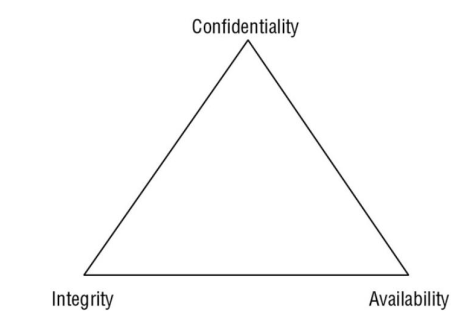
\includegraphics[width=.9\linewidth]{static/img/cysec/cia_triad.png}
\end{center}

\textbf{confidentiality}
\begin{itemize}
\item prevent unauthorized access to data
\item example: encryption, access controls
\end{itemize}

\textbf{integrity}
\begin{itemize}
\item protecting the reliability and correctness of data
\item example: intrusion detection systems (IDS), hash verification
\end{itemize}

\textbf{availability}:
\begin{itemize}
\item authorized subjects are granted timely and uninterrupted access to objects
\item example: redundancy, maintain reliable backups, prevent data loss or destruction
\end{itemize}


\textbf{nonrepudiation}: ensure that the subject is not able to
\begin{itemize}
\item deny having performed an action
\item deny that the event occurred
\end{itemize}
\textbf{accountability}
\begin{itemize}
\item being responsible or obligated for actions and results
\item nonrepudiation is an essential part of accountability
\end{itemize}

\subsection*{Data classification}
\label{sec:orgf24ed78}
\begin{itemize}
\item is used to determine how much effort, money and resources are allocated to protect the data
\end{itemize}
data states:
\begin{itemize}
\item \textbf{data at rest}: data on media such as HDDs, SSDs, SANs, \ldots{}
\item \textbf{data in transit}: data transmitted over a network
\item \textbf{data in use}: data processed by an application
\begin{itemize}
\item data can not be used in encrypted state
\end{itemize}
\end{itemize}

defining sensitive data:
\begin{itemize}
\item \textbf{Personally Identifiable Information (PII)}
\item \textbf{Protected Health Information (PHI)}
\item \textbf{Proprietary Data}
\begin{itemize}
\item any data that helps an organization to maintain a competitive edge
\end{itemize}
\end{itemize}

Government / military classification:
\begin{enumerate}
\item Top secret
\item Secret
\item Confidential
\item Sensitive but unclassified
\item Unclassified
\end{enumerate}

Commercial business / private sector classification:
\begin{enumerate}
\item Confidential / Private
\item Sensitive
\item Public
\end{enumerate}

destroying sensitive data:
\begin{itemize}
\item \textbf{erasing}
\begin{itemize}
\item normally deletes just the directory / catalog link to the data
\end{itemize}
\item \textbf{clearing / overwriting}
\begin{itemize}
\item preparing for reuse
\item write 1 character, write complement, write random bits
\end{itemize}
\item \textbf{purging}
\begin{itemize}
\item more intense form of clearing to prepare media for reuse in less secure environments
\item repeats the clearing process multiple times
\end{itemize}
\item \textbf{degaussing}
\begin{itemize}
\item create a strong magnetic field that erases data on some media
\item does not affect optical medias and SSDs
\end{itemize}
\item \textbf{destruction}
\begin{itemize}
\item destroy the media
\item crushing, shredding, \ldots{}
\end{itemize}
\end{itemize}

tracing or hiding sensitive data:
\begin{itemize}
\item \textbf{Steganography}
\begin{itemize}
\item practice of embedding a message within a file
\end{itemize}
\item \textbf{Watermarking}
\begin{itemize}
\item embedding an image / patter in paper that isn't readily perceivable
\item digital watermarks is a secretly embedded marker in a digital file
\end{itemize}
\end{itemize}

\subsection*{Threat}
\label{sec:orgc340374}
\textbf{threat}: any potential danger to an asset (intentional or accidental)

\textbf{threat actor / agent}
\begin{itemize}
\item script kiddies
\item organized crime groups
\item state sponsors / governments
\item hacktivists
\item terrorist groups
\end{itemize}

\textbf{threat intelligence}: knowledge about an existing threat to assets)

\textbf{threat event}:
\begin{itemize}
\item accidental and intentional exploitation's of vulnerabilities
\item can be natural or man made
\begin{itemize}
\item example: fire, earthquake, flood, system failure, human error, \ldots{}
\end{itemize}
\end{itemize}

\textbf{STRIDE thread model}
\begin{itemize}
\item \textbf{S}poofing: gain access to a system through the use of a falsified identiy
\item \textbf{T}ampering: any action resulting in unauthorized changer or manipulation of data
\item \textbf{R}epudiation: the ability of a user / attacker to deny having performed an action
\item \textbf{I}nformation disclosure: the revelation / distribution of private / confidential or controlled information to unauthorized entites
\item \textbf{D}enial of service (DoS): attack to prevent authorized use of a resource
\item \textbf{E}levation of privilege: a limited user account is transformed into an account with greater privileges / power / access
\end{itemize}

\subsection*{Vulnerability}
\label{sec:orgfd080c7}
\textbf{Vulnerability}: weakness in an asset
\begin{itemize}
\item Common Vulnerabilities and Exposures (\emph{CVE})
\end{itemize}

\textbf{Exploit}: software / sequence of commands the take advantage of a vulnerability

\subsection*{Risk management}
\label{sec:orgdd86440}
\textbf{Risk management}:
\begin{itemize}
\item develop information security strategies
\item reduce risk (to an acceptable level)
\item identifying factors, evaluating factors, implement cost-effective solutions for mitigating / risk reduction
\end{itemize}

\textbf{Countermeasure}: any action / product that reduces risk through elimination / lessening of a thread / vulnerability

\textbf{Risk analysis}:
\begin{itemize}
\item process by which the goals of risk management arch achieved
\item evaluation of all assets
\item examining for risk
\item evaluating each threat
\item assessing the cost of countermeasures
\end{itemize}

\textbf{Asset Valuation}: dollar value assigned to an asset based on
\begin{itemize}
\item cost
\item non monetary expenses
\end{itemize}

\textbf{Exposure}: possibility for an asset loss because of a threat

\textbf{Risk}: possibility that something could happen to damage, destroy or disclose data / resources

\textbf{Attack}: exploitation of a vulnerability by a threat agent

\textbf{Breach}: occurrence of a security mechanism being bypassed 


\begin{center}
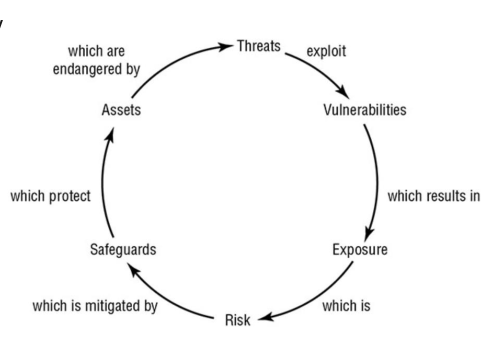
\includegraphics[width=.9\linewidth]{static/img/cysec/risk_terminology.png}
\end{center}


\subsubsection*{Quantitative risk analysis}
\label{sec:org1546604}
\begin{enumerate}
\item \textbf{Exposure factor (EF)}: percentage of the overall asset value loss

\item \textbf{Single loss expectancy (SLE)}: cost associated with a single realized risk
\begin{itemize}
\item SLE = asset value (AV) * exposure factor (EF)
\end{itemize}

\item \textbf{Annualized rate of occurrence (ARO)}: the expected frequency with which threat / risk will occur within a single year

\item \textbf{Annualized loss expectancy (ALE)}: the possible yearly cost against a specific asset
\begin{itemize}
\item ALE = single loss expectancy (SLE) * annualized rate of occurrence (ARO)
\end{itemize}

\item \textbf{Annualized loss expectancy with a safeguard (ALE)}:
\begin{itemize}
\item the possible yearly cost against a specific asset with an new EF and ARO
\item EF stays normally the same, ARO should be smaller (go to zero)
\end{itemize}

\item \textbf{Safeguard Costs}: assign each safeguard with a deployment value = ACS
\begin{itemize}
\item ACS (Annual cost of the safeguard)
\end{itemize}

\item \textbf{Calculating safeguard cost/benefit}:
\begin{itemize}
\item ALE before safeguard - ALE with safeguard - annual cost of safeguard (ACS) = value of the safeguard to the company
\item result < 0: safeguard is not a financially responsible choice
\item result > 0: this is the amount of money which could be saved when deployed (rate of occurrence is not a guarantee of occurrence)
\end{itemize}
\end{enumerate}

\begin{center}
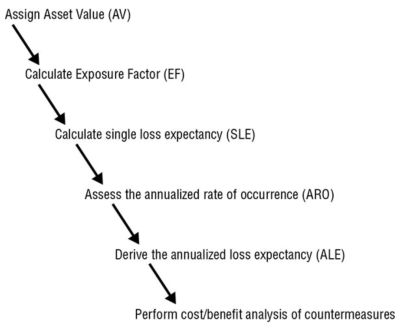
\includegraphics[width=.9\linewidth]{static/img/cysec/quantitative_risk_analysis.png}
\end{center}

\subsubsection*{risk treatments methods}
\label{sec:orgce3da03}
\textbf{Risk Mitigation}: implement safeguards to eliminate vulnerabilities or block threats

\textbf{Risk Assignment}: placement of the cost of loss onto another entity / organization (e.g. outsourcing)

\textbf{Risk Acceptance}: when countermeasures cost more than the possible loss you can accept the risk

\textbf{Risk Deterrence (en für Abschreckung)}: implementing deterrents for would-be violators of security and policy (e.g camera, motion detection)

\textbf{Risk Avoidance}: select alternate options / activities that have less associated risk

\textbf{Risk Rejection}: reject risk / ignore risk (unacceptable)

\textbf{Residual risk}: the risk witch is left after implementing the countermeasures

\subsection*{Privacy}
\label{sec:org803030c}
\textbf{Privacy}: the right of the individual to control their personal data

\textbf{pseudonymization}: replacing data elements with pseudonyms
\begin{itemize}
\item can be reversed to make data meaningful
\end{itemize}

\textbf{Anonymization}: removing all relevant data so that it is impossible to identify the original subject / person

\begin{itemize}
\item USA PATRIOT Act
\item EU GDPR
\end{itemize}

\section*{Week 02 - Identity and Access Management (IAM)}
\label{sec:org97a6a8a}
\subsection*{Controlling access to assets}
\label{sec:org0265324}
\begin{itemize}
\item \textbf{access control}
\begin{itemize}
\item any hardware, software, administrative policy / procedure that controls access to resources
\end{itemize}

\item \textbf{Subject}
\begin{itemize}
\item an active entity that access a passive object
\item[{examples}] users, programs, computers, \ldots{}
\end{itemize}

\item \textbf{Object}
\begin{itemize}
\item a passive entity that provides information to active subjects
\item[{example}] files, databases, services, storage media, \ldots{}
\end{itemize}
\end{itemize}


\begin{center}
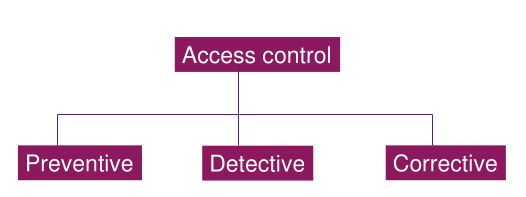
\includegraphics[width=.9\linewidth]{static/img/cysec/primary_access_control_types.png}
\end{center}

\begin{itemize}
\item \textbf{Preventive Access Control}
\begin{itemize}
\item preventive control to stop unwanted / unauthorized activity from occurring
\item[{example}] fences, locks, alarm system, \ldots{}
\end{itemize}

\item \textbf{Detective Access Control}
\begin{itemize}
\item attempts to discover / detect unwanted / unauthorized activity
\item can discover the activity only after it has occurred
\item[{example }] security guards, motion detectors, \ldots{}
\end{itemize}

\item \textbf{Corrective Access Control}
\begin{itemize}
\item modifies the environment to return system to normal after an unwanted / unauthorized activity has occurred
\item try to correct problems that occurred because of a security incident
\item[{example}] rebooting system, backup and restore plans, \ldots{}
\end{itemize}
\end{itemize}


\begin{center}
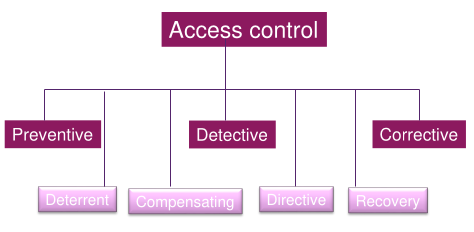
\includegraphics[width=.9\linewidth]{static/img/cysec/other_access_control_types.png}
\end{center}

\begin{itemize}
\item \textbf{Deterrent}
\begin{itemize}
\item discourage violation of security policies
\item the subject decides itself not to take an unwanted action
\item[{example}] security-awareness training, locks, security camera
\end{itemize}

\item \textbf{Compensating}
\begin{itemize}
\item provide various options to other existing controls to aid
\end{itemize}

\item \textbf{Directive}
\begin{itemize}
\item controls to force compliance with security policies
\item[{example}] security policy requirements / criteria, escape route exit signs, monitoring, \ldots{}
\end{itemize}

\item \textbf{Recovery}
\begin{itemize}
\item extension to corrective controls
\item have more advanced abilities
\item[{example}] backups and restores, fault-tolerant drive systems
\end{itemize}
\end{itemize}


\begin{itemize}
\item \textbf{Physical controls}
\begin{itemize}
\item items you can physically touch
\item prevent, monitor or detect contact with systems / areas
\item[{example}] guards, fences, locked doors, \ldots{}
\end{itemize}

\item \textbf{Technical / logical controls}
\begin{itemize}
\item hardware / software used to manage access
\item provide protection for resources / systems
\item[{example}] authentication methods, encryption, firewalls, \ldots{}
\end{itemize}

\item \textbf{Administrative controls}
\begin{itemize}
\item policies and procedures defined by organizations security policy
\item also known also management controls
\item[{example}] policies, background checks, data classifications and labeling, \ldots{}
\end{itemize}
\end{itemize}

\subsection*{The steps of access control}
\label{sec:org93873c9}
\begin{center}
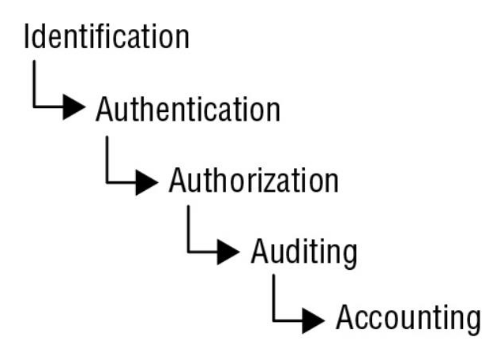
\includegraphics[width=.9\linewidth]{static/img/cysec/steps_of_access_control.png}
\end{center}

\subsubsection*{Identification}
\label{sec:org888772d}
\begin{itemize}
\item process of subject claiming an identity (e.g. username)
\end{itemize}

\subsubsection*{Authentication}
\label{sec:org4608d78}
\begin{itemize}
\item process of verifying that the claimed indent is valid (e.g. with password)

\item type of authentication
\begin{itemize}
\item password phrases
\item cognitive password
\item smart cards
\item tokens
\item (a)synchronous dynamic password tokens
\item onetime password generators
\item TOTP (Time-based One-time password)
\item HOTP (HMAC-based One-time password)
\end{itemize}

\item authentication factors
\begin{itemize}
\item type 1: \textbf{something you know}
\begin{description}
\item[{example}] password, PIN, passphrases
\end{description}
\item type 2: \textbf{something you have}
\begin{description}
\item[{example}] smart card, hardware token, memory card
\end{description}
\item type 3: \textbf{something you are / you do}
\begin{description}
\item[{example}] fingerprints, retina patterns, palm topology
\end{description}

\item additional factors
\begin{itemize}
\item \textbf{somewhere you are} (geographic location)
\item \textbf{somewhere you aren't} (geographic location)
\end{itemize}
\end{itemize}
\end{itemize}

\subsubsection*{Authorization}
\label{sec:orgd237d76}
\begin{itemize}
\item process ensures that the access to an object is possible with the rights and privileges

\item access control models
\begin{itemize}
\item \textbf{Discretionary Access Control (DAC)}
\begin{itemize}
\item every object has an owner
\item owner can grant / deny access to any other subjects
\item NTFS / MS used this
\end{itemize}

\item \textbf{Role Based Access Control}
\begin{itemize}
\item permissions are not assigned directly to users
\item users are placed in roles
\item privileges are assigned to roles
\end{itemize}

\item \textbf{Rule Based Access Control}
\begin{itemize}
\item global rules that are applied to all subjects
\item firewall uses often this type
\end{itemize}

\item \textbf{Attribute Based Access Control}
\begin{itemize}
\item uses of rules that can include multiple attributes
\end{itemize}

\item \textbf{Mandatory Access Control}
\begin{itemize}
\item uses of label applied to both subjects and objects
\item user has label top-secret can access objects label top-secret
\end{itemize}

\item \textbf{Implicit deny}
\begin{itemize}
\item as long as not explicit allowed it is denied
\end{itemize}

\item \textbf{Constrained Interface}
\begin{itemize}
\item UI is rendered based on subjects privileges
\end{itemize}

\item \textbf{Access Control Matrix}
\begin{itemize}
\item table that includes subjects, objects and assigned privileges
\item ACL are object focused and identify access granted to subjects for any object
\end{itemize}

\item \textbf{Capability Table}
\begin{itemize}
\item similar to Access Control Matrix
\item Capability tables are subject focused and identify the objects that subjects can access
\end{itemize}

\item \textbf{Content-Dependent Control}
\begin{itemize}
\item restrict access to data based on the content within an object
\item database view is an example for content dependent control
\end{itemize}

\item \textbf{Context-Dependent Control}
\begin{itemize}
\item requires specific activity before granting users access
\item users add items to the shopping cart and then pays for it. He can't pay before something is in the cart
\end{itemize}
\end{itemize}
\end{itemize}


\begin{itemize}
\item Principles
\begin{itemize}
\item \textbf{Need to Know}
\begin{itemize}
\item grant only access to what the subject need
\item subjects has label classified, object has label classified but when subject don't need this object for it's work it shouldn't have access
\end{itemize}

\item \textbf{Least Privilege}
\begin{itemize}
\item grant only this privileges they need to perform their work
\item write, create alter or delete data
\end{itemize}

\item \textbf{Separation of Duties and Responsibilities}
\begin{itemize}
\item no single person should have total control over critical function / system
\end{itemize}
\end{itemize}
\end{itemize}

\subsubsection*{Auditing}
\label{sec:orgb40a6af}
\begin{itemize}
\item recording activities of a subject and its objects
\end{itemize}

\subsubsection*{Accounting}
\label{sec:org3cc42d4}
\begin{itemize}
\item linking a human to the activities of an online identity through auditing, authorization, authentication and identification
\end{itemize}

\subsection*{The common access control attacks}
\label{sec:org4eeb27b}
\begin{itemize}
\item \textbf{Access Aggregation Attack (passive attack)}
\begin{itemize}
\item collect multiple non sensitive data and aggregating them to learn sensitive data
\end{itemize}

\item \textbf{Password Attacks (Brute-force attack)}
\begin{itemize}
\item attacks against online accounts
\item steal account database and crack the passwords offline
\end{itemize}

\item \textbf{Dictionary Attacks (Brute-force attack)}
\begin{itemize}
\item attempt to discover passwords by using every possible password in a predefined databases
\end{itemize}

\item \textbf{Birthday Attack (Brute-force attack)}
\begin{itemize}
\item finding collisions in hashes
\end{itemize}

\item \textbf{Rainbow Table Attacks}
\begin{itemize}
\item similar to dictionary attacks but the passwords are precomputed hashes
\end{itemize}

\item \textbf{Sniffer Attacks}
\begin{itemize}
\item capture traffic from the network
\end{itemize}

\item \textbf{Spoofing Attacks}
\begin{itemize}
\item pretending to be something / someone else
\end{itemize}

\item \textbf{Social Engineering Attacks}
\begin{itemize}
\item gain information over social interacting with other people
\end{itemize}

\item \textbf{Shoulder surfing}
\begin{itemize}
\item tries to look over the shoulder of target
\item special form of social engineering
\end{itemize}

\item \textbf{Phishing}
\begin{itemize}
\item Spear phishing
\begin{itemize}
\item targeted to a specific group of users (e.g. employees within a specific organization)
\end{itemize}

\item Whaling
\begin{itemize}
\item variant of phishing targeting high-level executives (CEOs)
\end{itemize}

\item Vishing
\begin{itemize}
\item like phishing but over instant messaging and VoIP
\end{itemize}
\end{itemize}
\end{itemize}

\subsection*{Protection mechanisms}
\label{sec:org03cd88a}
\begin{itemize}
\item Data hiding
\begin{itemize}
\item store data in a logical storage part where the subject has no access => data is not visible to the subject
\end{itemize}

\item security through obscurity
\begin{itemize}
\item idea of not informing about an object being present and hoping the subject will not discover the object
\item does not implement any form of protection. It hopes something important is not discovered
\end{itemize}

\item Encryption
\begin{itemize}
\item the art and science of hiding the meaning of a communication from unintended recipients
\end{itemize}
\end{itemize}

\section*{{\bfseries\sffamily TODO} Week 03 - Linux}
\label{sec:org550bfa2}
\section*{Week 04 - Symmetric and key exchange}
\label{sec:org2d7ae86}
\subsection*{Cryptography concepts}
\label{sec:org1b98833}
\begin{itemize}
\item \textbf{plaintext message}: message before coded into a form

\item \textbf{ciphertext}: cryptographic algorithm was used on a plaintext message

\item \textbf{cipher}: encryption algorithm

\item \textbf{cryptographic key}: a (large) number

\item \textbf{one-way functions}: mathematical operation that produces easily output values but it makes impossible to retrieve the input value

\item \textbf{reversibility}:

\item \textbf{Nonce}: Number only used once
\begin{itemize}
\item can be a counter
\item is public
\item used to make sure the key is not re-used twice
\end{itemize}

\item \textbf{Initialization vector (IV)}: a random bit string
\begin{itemize}
\item same length as block size
\item is XORed with the message
\item used to create unique ciphertext with the same key
\end{itemize}

\item \textbf{Confusion}: relationship between plain text and key is complicated
\begin{itemize}
\item substitution of bytes adds confusion
\end{itemize}

\item \textbf{Diffusion}: change in plaintext results in multiple changes in the ciphertext
\begin{itemize}
\item small change in input => big change on the output
\item permutation of bytes adds diffusion
\end{itemize}

\item \textbf{Kerckhoffs's Principle}: a cryptographic system should be secure even if everything about the system, except the key, is public knowledge

\item \textbf{SP-Network}: algorithm that uses repeated substitution and permutation operations

\item \textbf{One time pad}: unbreakable cipher
\begin{itemize}
\item message length = key length, XOR key with message
\item perfect secrecy
\item but not practicable (1GB file needs 1GB key)
\end{itemize}
\end{itemize}

\subsection*{Symmetric cryptography}
\label{sec:org54aeb73}
\begin{itemize}
\item symmetric key algorithms 
\begin{itemize}
\item uses \textbf{shared secrect} key (requireds a secure method of exchanging the key)
\begin{itemize}
\item used by all parties for encryption / decryption
\end{itemize}
\item large sized keys => verry difficult to break
\item only used for \textbf{confidentiality}
\item does not implement \textbf{nonrepudiation}
\item does not implement \textbf{message integrity}
\item[{pro}] extremley fast, many CPUs have AES instruction set
\end{itemize}

\item \textbf{stream cipher}
\begin{itemize}
\item one-time pad approximation with infinite pseudo random key stream
\item works on messages of any length
\item[{pro}] fast and low memory footprint
\item[{pro}] can seek to any location in the stream
\item[{con}] never reuse key + nonce
\item[{con}] do not protect the ciphertext (no guaranteed integrity)
\end{itemize}

\item \textbf{block cipher}
\begin{itemize}
\item take input of a fixed size; return output of same size
\item transformation from message to cipher trought confusion / diffusion
\item normally a SP-Network
\item AES is a SP-Network
\begin{itemize}
\item almost everything uses AES
\end{itemize}
\end{itemize}

\item \textbf{basic substitution box}
\begin{itemize}
\item input is substituted
\end{itemize}

\item \textbf{basic permutation box}
\begin{itemize}
\item bits will be rearranged
\end{itemize}
\end{itemize}

\subsubsection*{AES}
\label{sec:orgdbf76ac}
\begin{itemize}
\item \textbf{AES}: standard built arround the \textbf{Rijndael algorithm}
\begin{itemize}
\item AES = \textbf{A}dvanced \textbf{E}ncryption \textbf{S}tandard
\item SP-Network with 128-bit block size
\begin{itemize}
\item 10, 12, 14 rounds
\item SubBytes, ShiftRows, MixColumns, Key Addition
\end{itemize}
\end{itemize}
\end{itemize}


\begin{center}
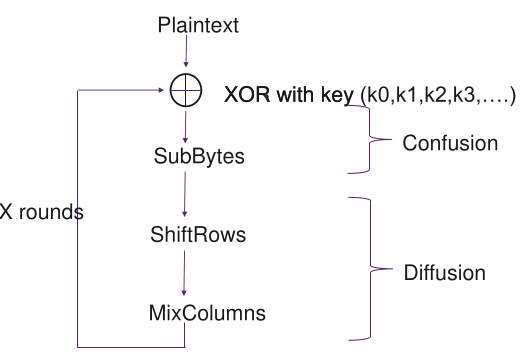
\includegraphics[width=.9\linewidth]{static/img/cysec/aes_network.png}
\end{center}

\subsubsection*{Mode of operations of block ciphers}
\label{sec:org6a6d8da}
\begin{itemize}
\item \textbf{Electronic Code Block (ECB)}
\begin{itemize}
\item just encrypt each block one after another
\item ECB is not not recommended
\end{itemize}

\item \textbf{Cipher Block Chaining (CBC)}
\begin{itemize}
\item XOR output of each cipher block with the next input
\item not parallelizable
\item betterthan ECB

\begin{center}
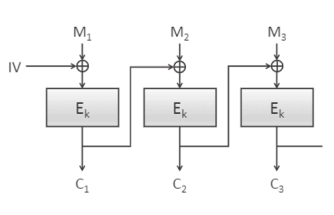
\includegraphics[width=.9\linewidth]{static/img/cysec/cbc_mode.png}
\end{center}
\end{itemize}

\item \textbf{Counter Mode (CTR)}
\begin{itemize}
\item encrypting a counter to produce a stream cipher
\item parallelizable
\item convert block cipher into a stream

\begin{center}
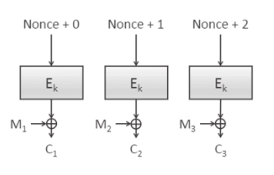
\includegraphics[width=.9\linewidth]{static/img/cysec/ctr_mode.png}
\end{center}
\end{itemize}
\end{itemize}

\subsection*{Diffie-Hellman Key exchange}
\label{sec:org1de70ac}
\subsubsection*{discrete logarithms problem}
\label{sec:org7c44f49}
\begin{align*}
  a^b &= c (\text{mod} n) \\
  b &= dlog_{a,n}(c) \\
\\
  7^2 &= 4 (\text{mod} 9) \\
  2 &= dlog_{7,9}(4)
\end{align*}
\begin{itemize}
\item to calculate the log is very difficult => brute force
\end{itemize}

\subsubsection*{Diffie-Hellman}
\label{sec:orga47c555}
\begin{enumerate}
\item both sites agree on parameter p (prime) and generator g (prime)
\item Alice and Bob select randomly their private values \textbf{a} and \textbf{b}
\begin{enumerate}
\item \(1 < a, b < p\)
\end{enumerate}
\item calculate public key
\begin{enumerate}
\item \(g^a mod p\) bzw. \(g^b mod p\)
\end{enumerate}
\item Swap public keys over the internet
\item combining public key with own private key
\begin{enumerate}
\item \((g^b)^a \text{mod }p = g^{ab}\text{mod }p\)
\item \((g^a)^b \text{mod }p = g^{ab}\text{mod }p\)
\end{enumerate}
\item Shared key = pre-master secret, used to derive session keys
\end{enumerate}


\begin{itemize}
\item \textbf{Emphemeral mode}
\begin{itemize}
\item new key exchange for evey new session (PERFECT FORWARD SECRECY)
\item Re-using a key doe's not make sense when just generate new ones
\item not necessarily every message (but pretty often)
\begin{itemize}
\item if someone is sniffing the traffic and breaking the keys, he don't get any of the previous messages
\item DH provides self-healing property
\end{itemize}
\end{itemize}
\end{itemize}

\subsubsection*{Elliptic Curve Cryptography (ECDHE)}
\label{sec:org27dafa0}
\begin{itemize}
\item \textbf{ECDHE}
\begin{itemize}
\item drop in replacement for regular Diffie-Hellman
\item becoming the standard
\item elliptic curve discrete logarithm problem (ECDLP) is slight more difficult than discret logarithm
\end{itemize}

\item elliptic curve needs a lot less bits for same security
\end{itemize}

\section*{Week 05 - Assymetric and hash functions}
\label{sec:org31e3266}
\subsection*{RSA}
\label{sec:org780ed4d}
\begin{itemize}
\item two use cases
\begin{enumerate}
\item encryption: encrypt with others public key => decrypt with own private key
\item signing: encrypt with own private key => decrypt with public key
\end{enumerate}

\item public key (e, n), private key (d)
\begin{itemize}
\item e usually small (2, 3) for efficiency
\item n is very lager number by multiply two primes number together (\(p_1 \cdot p_2\))
\end{itemize}

\item based on \textbf{factoring problem}:
\begin{itemize}
\item hard of factoring the product of two large prime numbers => \textbf{time complexity}
\end{itemize}

\item \textbf{one-way trapdoor function}:
\begin{itemize}
\item no way to undo the encryption function unless you know the trapdoor
\item known the factors of \textbf{n} is the trapdoor
\end{itemize}

\item Encrypt message witch public key (e,n)
\begin{itemize}
\item \(c=m^e \text{mod } n\)
\end{itemize}
\item Decrypt message with private key (d)
\begin{itemize}
\item \(m = c^d \text{mod }n\)
\end{itemize}

\item \textbf{\(\Phi\) -Funktion}:
\begin{itemize}
\item n positive integer, m prime
\item \(m^{\Phi}(n) = 1 \text{mod } n\)
\item \(d = \frac{(k \cdot \Phi(n) + 1)}{e}, k \in \mathbb{Z}\)
\end{itemize}

\item generating key pairs is time-consuming, should be done rarely
\begin{itemize}
\item e is almost always 3 or 65537
\end{itemize}
\end{itemize}


\subsubsection*{Build parameters}
\label{sec:orgeb714a7}
\begin{enumerate}
\item Choose p\textsubscript{1} and p\textsubscript{2}
\begin{enumerate}
\item \(n = p_1 \cdot p_2\)
\item n is public, p\textsubscript{1}, p\textsubscript{2} private
\end{enumerate}
\item Calculate \(\Phi\)(n)
\begin{enumerate}
\item \(\Phi(n) = \Phi(p_1 \cdot p_2) = \Phi(p_1)\cdot\Phi(p_2) = (p_1 - 1) \cdot (p_2 -1)\)
\end{enumerate}
\item Choose exponents e and
\begin{enumerate}
\item choose e freely
\item \(d = \Phi(n) - \lfloor\frac{\Phi(n)}{e}\rfloor \cdot\)
\item Verification: \(d = \frac{k\cdot\Phi(n)+1}{e}\)
\end{enumerate}
\end{enumerate}

\subsection*{Encrypting using RSA}
\label{sec:org3b5e0b2}
\begin{itemize}
\item is very weak for short messages
\begin{itemize}
\item padding added to short messages (Optimal asymmetric Encryption padding - OAEP)
\item OAEP: pseudo random padding that introduce an IV process and hashes it
\item receiver has to do the exact same padding to match the messages
\end{itemize}
\item Encryption using RSA is not very common (slow)
\end{itemize}

\subsection*{Signing using RSA}
\label{sec:orgde9bd8b}
\begin{itemize}
\item Same process as normal encryption. Just encrypt message with own private key

\item digital signature often sent as a challenge (prove its identity)
\begin{enumerate}
\item client sent message to server
\item server sign it with its private key
\item client decrypt the signed message using public key
\item compares original messages with message from server
\end{enumerate}
\end{itemize}


\begin{enumerate}
\item message is first hashed
\item hash is signed and sent with message
\item the receiver hashes message, decrpyt the signature compare hashes
\end{enumerate}


\begin{itemize}
\item \textbf{DSA}: Digital Signature Algorithm:
\begin{itemize}
\item RSA in some years to slow => DSA will become standard
\item DAS only for signing
\end{itemize}
\end{itemize}

\subsection*{The hash function}
\label{sec:org102c8ed}
\begin{itemize}
\item takes message of any length, returns hash of fixed length
\item hash functions iterative jumble blocks of messages after another
\item output should not look like based on input
\item small changes input => big changes output
\end{itemize}

\begin{center}
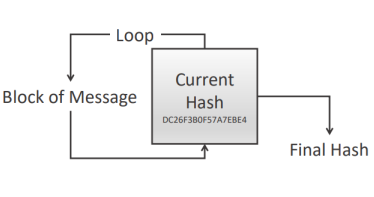
\includegraphics[width=.9\linewidth]{static/img/cysec/hash_loop_function.png}
\end{center}


\begin{itemize}
\item strong hash function:
\begin{enumerate}
\item quick, but not too quick
\item it has to introduce diffusion
\item no possible to reverse
\item given messages with its hash, no other messages hashes to the same thing
\begin{itemize}
\item that is a collision
\end{itemize}
\item we can't find tow messages with same hash
\end{enumerate}
\end{itemize}


\begin{itemize}
\item \textbf{SHA-2 / SHA-3}
\begin{itemize}
\item standard
\item shouldn't be used for passwords (they are to fast)
\end{itemize}

\item \textbf{PBKDF2 (Password Based Key Derivation Function 2)}:
\begin{itemize}
\item should used for passwords / login
\item useless for everything else
\end{itemize}
\item \textbf{Bcrypt}
\begin{itemize}
\item alternative to PBKDF2
\end{itemize}
\end{itemize}


\begin{itemize}
\item Usage of Hashes:
\begin{enumerate}
\item Digital signature
\item Symmetric cryptography is vulnerable to message tampering
\begin{itemize}
\item Hashes let us ensure that messages hasn't changed
\item \textbf{Message Authentication Code (MAC)}
\item Hash(K|C) is append to the ciphertext C
\item if receiver hasshes key and ciphertext and its equal to the receiver messages hash, nothing changed
\end{itemize}
\end{enumerate}

\item \textbf{HMAC}
\begin{itemize}
\item Split key in two
\item hash twice with each key
\end{itemize}
\end{itemize}

\begin{center}
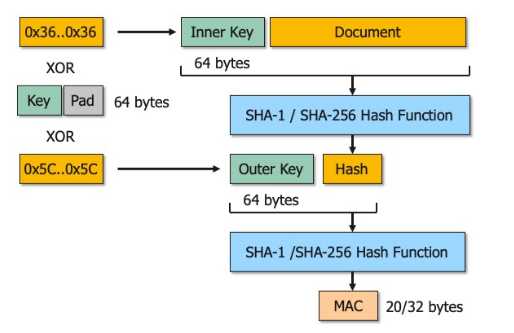
\includegraphics[width=.9\linewidth]{static/img/cysec/hmac.png}
\end{center}

\section*{Week 06 - Complete cryptography systems}
\label{sec:orgdcb2b49}
\subsection*{Public cryptography}
\label{sec:orgc62ef8d}
\begin{itemize}
\item \textbf{Digital certificates}
\begin{itemize}
\item digital signature proves access to private key (doesn't prove trust)
\item digital certificates verify ownership of a public key
\end{itemize}
\end{itemize}


\begin{itemize}
\item \textbf{Certificate Issuance}
\begin{enumerate}
\item generate RSA / DSA private and public key
\item creates a \textbf{Certificate Signing Request (CSR)}
\begin{itemize}
\item CSR is a certificate which has to be verified
\end{itemize}
\item CSR is sent to a \textbf{Certification Authority (CA)}
\item CA does some identification checks
\item CA creates and signs the certificate with its private key
\end{enumerate}

\item \textbf{Certificate Use}
\begin{enumerate}
\item decrypt signature from server with public key from certificate
\item in order to trust the public key you have to verify the digital signature at the bottom of the certificate
\end{enumerate}

\item \textbf{Chain of trust}
\begin{itemize}
\item to trust server a, we have to trust the issuer of the certificate
\item to trust the issuer, we have to trust the next issuer; and so on
\item root certificates are trusted because built into OS / Browser / etc.
\end{itemize}
\end{itemize}

\subsection*{Complete cryptographic systems}
\label{sec:org7861730}
\begin{itemize}
\item \textbf{Authenticated Encryption with associated data (AEAD)}
\begin{itemize}
\item guarantee the confidentiality and integrity using MAC
\item encrypted message
\item message and additional data authenticated
\end{itemize}

\item \textbf{AES Galois Counter Mode (GCM)}
\begin{itemize}
\item it's a AEAD protocol
\item AES in CTR and Galois Message Authentication Code (GCM) as MAC / GMAC
\end{itemize}

\item \textbf{ChaCha20\textsubscript{Poly1305}}
\begin{itemize}
\item it's a AEAD protocol
\item ChaCha20 stream cipher, Poly1305 a MAC
\item used on mobile phones, on CPUs without AES instructions ChaCha20 is faster
\end{itemize}

\item Protocol Handshakes
\begin{enumerate}
\item Handshake phase
\begin{itemize}
\item Agree on set of cryptographic protocols
\item perform key exchange, obtain session keys, IVs, \ldots{}
\item verify authentication using public key
\end{itemize}

\item Transport / Record Phase
\begin{itemize}
\item encrypt message using cipher
\item include MAC to verify integrity
\end{itemize}
\end{enumerate}

\item Common Protocol Issues
\begin{itemize}
\item not secured with MAC
\item no time-stamp or counter included
\item no public key authentication used
\item reuse of Nonces or IVs
\end{itemize}
\end{itemize}

\section*{Week 07 - TLS}
\label{sec:orgb597ed5}
\subsection*{Introduction to TLS}
\label{sec:org7aca791}
\begin{itemize}
\item OSI Layer 4+
\item based on TCP
\item responsible for
\begin{itemize}
\item fragmentation into TLS PDUs
\item compression of PDUs before encryption
\item authentication of PDUs
\item encryption of PDUs
\end{itemize}
\item SSL (Secure Socket Layer) previous name, now TLS (Transport Layer Security)
\end{itemize}


\subsubsection*{TLS Architecture}
\label{sec:orgdc896e8}
\begin{itemize}
\item \textbf{TLS connection}
\begin{itemize}
\item transport that provides a suitable type of service
\item peer-to-peer
\item transient
\item is associated with one session
\end{itemize}

\item \textbf{TLS session}
\begin{itemize}
\item association between a client and server
\item defines a set of cryptographic security parameters (shared over multiple connections)
\item used to avoid expensive negotiation of new parameters
\end{itemize}

\item \textbf{Connection State Definition}
\begin{itemize}
\item MAC
\item key
\item IV
\item sequence number
\end{itemize}

\item \textbf{Session State Definition}
\begin{itemize}
\item Session identifier
\item peer certificate (may be null)
\item compression method
\item cipher spec
\item master secret (48-byte)
\item is reusable flag
\end{itemize}
\end{itemize}

\subsubsection*{History}
\label{sec:org377a962}
\begin{itemize}
\item SSL 1 - TLS 1.0 shouldn't used (broken)
\item TLS 1.1 - TLS 1.3 are OK
\item TLS 1.3 - Clean up
\begin{itemize}
\item remove unsafe / unused features
\item performance: 1-RTT and 0-RTT
\item improve security with modern techniques
\item encrypt more of the protocol, (almost all handshakes messages are encrypted)
\item backwards compatibility
\end{itemize}
\end{itemize}


\subsection*{TLS Protocol}
\label{sec:orgf02e0f5}
\begin{itemize}
\item Record header
\begin{itemize}
\item type (which TLS message is sent, 1 byte)
\item version (2 bytes)
\item length (2 bytes)
\end{itemize}

\item application data
\begin{itemize}
\item max 2\textsuperscript{14} bytes per segment
\item one TLS-message can be longer than one segment
\end{itemize}

\item TLS-Records types:
\begin{itemize}
\item \textbf{TLS Handshake} (ClientHello, ServerHello, Certificate, ServerHelloDone)
\item \textbf{TLS Change CipherSpec}
\item \textbf{TLS Alert} (Warning, Fatal, Session is closed immediately)
\item \textbf{TLS Application Data} (Transmission of encrypted payload)
\end{itemize}
\end{itemize}

\subsubsection*{TLS Handshake}
\label{sec:orga5f3de5}
\begin{itemize}
\item allows authentication
\item negotiate encryption / MAC algorithms
\item negotiate cryptographic keys
\item 4 phases
\end{itemize}


\begin{enumerate}
\item Phase
\begin{enumerate}
\item sent ClientHello with random bytes R\textsubscript{c}
\item server response with ServerHello and random bytes R\textsubscript{s}
\end{enumerate}
\item Phase
\begin{enumerate}
\item server normally sends now it's X.509 certificate in a \textbf{Certificate} message
\item optional: \textbf{ServerKeyExchange} containing the server part of DH secret
\item optional: \textbf{Certificate Request} to authenticate client is send from server
\item after the server hello phase the server sends a \textbf{ServerHelloDone} message
\end{enumerate}
\item Phase
\begin{enumerate}
\item client sent it's certificate if requested in a \textbf{Certificate} message
\item if certificate from server received encrypt random premaster secret with public key from certificate and set it to the server in a \textbf{ClientKeyExchange} message. or send it's DH parameters
\end{enumerate}
\item Phase
\begin{enumerate}
\item Client sends \textbf{ChangeCipherSpec} announcing that now the new parameters are used followed by \textbf{Finished} message
\item Server does the same on it's site
\end{enumerate}
\item Application data can be transmitted
\end{enumerate}


\begin{itemize}
\item \textbf{Forward secrecy (FS)}
\begin{itemize}
\item FS protects past sessions against future compromises of keys or passwords
\item over RSA public key encryption has no perfect forward secrecy
\item over DH key exchange with perfect forward secrecy
\end{itemize}

\item \textbf{Computing TLS master secret}
\begin{enumerate}
\item Pre master secret has to be exchanged
\item master secret is calculated by both parties
\begin{itemize}
\item for pre master secret exchange can RSA or DH be used
\item RSA, client generates 48-byte pre master key and sent it encrypted with public key of server back
\item DH: normal DH key exchange
\end{itemize}
\end{enumerate}
\end{itemize}


\subsubsection*{TLS Alert protocol}
\label{sec:org0cb8ba0}
\begin{itemize}
\item 2 bytes length
\item first byte: level - warning or fatal (fatal immediately termination)
\item second bytes: code that indicates the specific alert
\end{itemize}


\subsubsection*{TLS Session Resumption}
\label{sec:org084b9a7}
\begin{itemize}
\item instead of of negotiating new security parameter the previous session can be used
\begin{enumerate}
\item \textbf{ClientHello} with previous \textbf{Session ID}
\item if session is still in cache on server side the session is reused and \textbf{ChangeCipherSpec} and \textbf{Finished} is sent
\item client response with \textbf{ChangeCipherSpec} and \textbf{Finished}
\item If no match is found on server a full handshake is perfomred
\end{enumerate}
\end{itemize}


\subsubsection*{Heartbeat Protocol}
\label{sec:org2b4e9b1}
\begin{itemize}
\item runs on top of TLS Record protocol
\item assures the sender is still alive
\item generates activity across the connection during idle periods
\end{itemize}


\subsubsection*{SSL / TLS Attacks}
\label{sec:org2ee0469}
\begin{center}
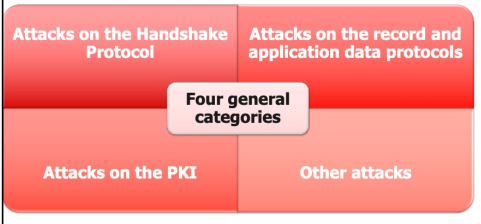
\includegraphics[width=.9\linewidth]{static/img/cysec/ssl_tls_attacks.png}
\end{center}


\subsection*{TLS 1.3}
\label{sec:org4a84e44}
\begin{itemize}
\item 1-RTT
\begin{itemize}
\item clients sends \textbf{ClientHello} with \textbf{KeyShare}
\item Server sends \textbf{ServerHello} with \textbf{KeyShare}, \textbf{ServerParameters} and \textbf{Authentication}
\item client sends \textbf{Authentication} and first \textbf{Application Data}
\end{itemize}

\item Cipher Suites
\begin{itemize}
\item Key Exchange:  DHE, ECDHE
\item Authentication: RSA, ECDSA, EdDSA
\item Cipher Suites:
\begin{itemize}
\item TLS\textsubscript{AES}\textsubscript{128}\textsubscript{GCM}\textsubscript{SHA256}
\item TLS\textsubscript{AES}\textsubscript{256}\textsubscript{GCM}\textsubscript{SHA384}
\item TLS\textsubscript{CHACHA20}\textsubscript{POLY1305}\textsubscript{SHA256}
\item TLS\textsubscript{AES}\textsubscript{128}\textsubscript{CCM}\textsubscript{SHA256} (IoT)
\item TLS\textsubscript{AES}\textsubscript{128}\textsubscript{CCM}\textsubscript{8}\textsubscript{SHA256} (IoT)
\end{itemize}
\end{itemize}
\end{itemize}

\section*{Week 08 - Advanced TLS}
\label{sec:org7fa63b2}
\subsection*{Public Key Infrastructure (PKI)}
\label{sec:org2aa13b8}
\begin{itemize}
\item \textbf{Public Key Infrastructure (PKI)}
\begin{itemize}
\item used to bind public key to an identity of a person / organization
\item registration process by a \textbf{Registration Authority (RA)}
\item issuance of a certificate by a \textbf{Certificate Authority (CA)}
\item CA can be validated by independent \textbf{Validation Authority (VA)}
\item artifact of binding is the \textbf{certificate}
\end{itemize}
\end{itemize}


\begin{center}
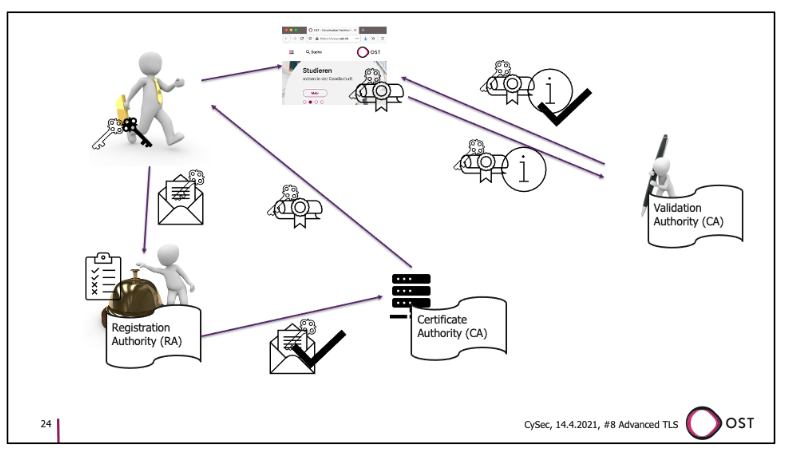
\includegraphics[width=.9\linewidth]{static/img/cysec/pki.png}
\end{center}
\subsection*{X.509 Certificates}
\label{sec:org6aea78c}
\begin{itemize}
\item standard for the format of public key certificates

\item public key certificate = digital / electronic certificate
\begin{itemize}
\item proving ownership of a public key
\item information about the key
\item identity of its owner (aka. \textbf{subject})
\item entity that has verified the certificate's content (aka. \textbf{issuer}
\end{itemize}

\item certificate quality
\begin{itemize}
\item \textbf{Domain Validated (DV)}
\begin{itemize}
\item check if owner has right to use the domain
\end{itemize}

\item \textbf{Organization Validated (OV)}
\begin{itemize}
\item after the company name, domain name and other information through the use of public databases is checked
\end{itemize}

\item \textbf{Extended Validation (EV)}
\begin{itemize}
\item only after a strict authentication producer is passed
\end{itemize}

\item \textbf{Qualified Website Authentication Certificate (QWAC)}

\item validity information
\begin{enumerate}
\item \textbf{Certificate Revocation List (CRL)}
\item \textbf{Online Certificate Status Protocol (OCSP)}
\end{enumerate}
\end{itemize}
\end{itemize}


\subsection*{Trust Service Providers - Certificate Authorities}
\label{sec:org6dd7112}
\begin{itemize}
\item \textbf{Trust Service Provider (TSP)}
\begin{itemize}
\item establish trust between communicating parties
\begin{itemize}
\item providing identity information
\item secure authentication
\item integrity protected communication
\item encrypted communication
\end{itemize}
\end{itemize}

\item \textbf{Certificate Issuance}
\begin{itemize}
\item \textbf{subscriber} prepares based on public key a \textbf{certificate signing request (CSR)}
\item the CA will register the request, verify data, and if everything OK => CSR turns into a X.509 certificate
\end{itemize}

\item CA hierarchy
\begin{itemize}
\item \textbf{Root CA} the last / first part of the chain of trust. Apps, Computers, Users trust the Root CA
\item \textbf{Issuing CA} issues certificate to end entities (Intermediate CA / Subordinate CA)
\item because of security / logical separation / flexibility these are roles are separated
\end{itemize}

\item \textbf{CA / Browser Forum (CA / B)}
\begin{center}
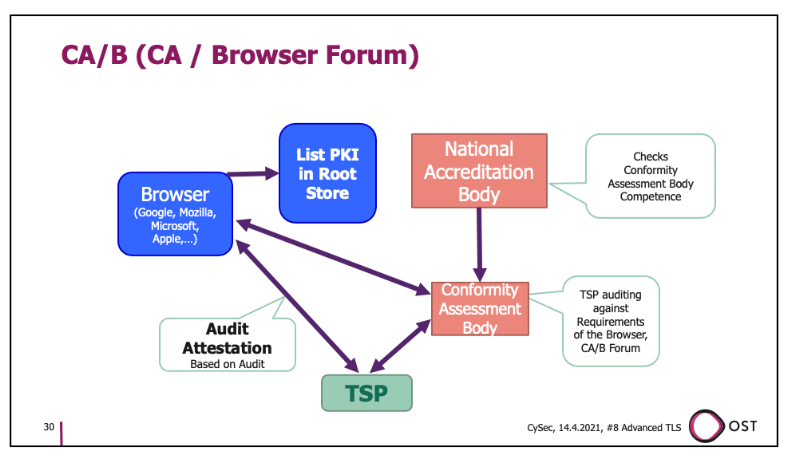
\includegraphics[width=.9\linewidth]{static/img/cysec/ca_b.png}
\end{center}

\item Principle elements of conformity assessment (How to become a TSP)
\begin{enumerate}
\item Stage: Document assessment
\begin{itemize}
\item technical, function, organizational security measures
\end{itemize}
\item Stage On-Site assessment
\begin{itemize}
\item verify implementation of security measures (including technical and pen testing)
\end{itemize}
\item Results report
\begin{itemize}
\item identification of the TSP, service and policy content and summary
\end{itemize}
\end{enumerate}
\end{itemize}


\begin{itemize}
\item \textbf{Certificate pinning}
\begin{itemize}
\item operators limit the who is allowed to issue a certificate for the domain (pin)
\item Pin the root
\item Pin the intermediate CA
\item Pin the end entity certificate (also called the \textbf{SSH model}
\end{itemize}
\end{itemize}

\section*{Week 09 - Authentication Protocols}
\label{sec:orge91b2c5}
\subsection*{Authentication Schemes}
\label{sec:org519e13f}
\begin{itemize}
\item Authentication Schemes Classification
\begin{enumerate}
\item A1. \textbf{Basic Authentication}: classical username / password pair transmitted clear
\begin{description}
\item[{cons}] prone to passive sniffing
\end{description}

\item A2. \textbf{One Time Passwords}: transmitted clear but used only once
\begin{description}
\item[{pros}] efficient means against passive sniffing attack
\item[{cons}] do not protect against active Main-In-the-Middle (MITM)
\end{description}

\item A3. \textbf{Challenge / Response}: function of password and one-time challenge
\begin{description}
\item[{pros}] efficient means against passive sniffing attack
\item[{cons}] do not protect against active Main-In-the-Middle (MITM)
\end{description}

\item A4. \textbf{Anonymous Key Exchange}: exchange credentials over unauthenticated secure channel
\begin{description}
\item[{pros}] algorithms like DH can be used to calculate a common secret
\item[{cons}] vulnerable to MITM because endpoint do not authenticate themselves
\end{description}

\item A5. \textbf{Zero-Knowledge Password Proofs}: does not permit offline-based password attacks
\begin{description}
\item[{pros}] Brute Force impossible because the DH parameters are random
\item[{cons}] password database on server could be stolen
\end{description}

\item A6. \textbf{Server Certificate plus User Authentication}: transmitting password over unilaterally authenticated secure channel (using DH and signature) 
\begin{description}
\item[{pros}] 

\item[{cons}] password database could be stolen from the server
\end{description}

\item A7. \textbf{Mutual Public Key Authentication}: bilateral use of public key signatures
\begin{description}
\item[{pros}] with client certificates no need to store user credentials, client certificates can be stores on an smart card protected by a PIN (strong 2-FA)
\item[{cons}] non besides the worst case of a root CA compromise
\end{description}
\end{enumerate}
\end{itemize}


\subsubsection*{A3. Challenge / Response}
\label{sec:org23d3db2}
\begin{itemize}
\item the proper way of authenticating over an insecure channel

\item \textbf{Challenge / Response based on MAC}
\begin{itemize}
\item Hash(id + challenge + random bytes client + clients password) is the MAC
\item if both the transmitted MAC and the server side calculated MAC is equal => authenticated
\end{itemize}

\item \textbf{Challenge / Response based on Digital Signatures}
\begin{itemize}
\item same idea as above
\item signature of Hash(ID, R\textsubscript{U}, R\textsubscript{S}) is append and compared
\end{itemize}
\end{itemize}


\begin{itemize}
\item Kerberos
\label{sec:orgf072ed5}
\begin{itemize}
\item \textbf{Key Distribution Center (KDC)}
\begin{itemize}
\item every principal has a secret master key (derived from login password) registered with the KDC
\item all master keys are stored in the KDC database, encrypted with the KDC master key
\end{itemize}

\item \textbf{Simplified Kerberos Protocol}
\begin{itemize}
\item algorithm 
\begin{enumerate}
\item Alice
\begin{enumerate}
\item Alice derive Master Key from Login password
\item Send encrypted time to the
\end{enumerate}
\item KDC
\begin{enumerate}
\item KDC decrypts time => valid?
\item Generate Session Key
\item Encrypt Session Key with Master Key from Alice
\item Encrypt Session Key and name (alice) with master key from Bob (ticket)
\item Send session key and ticket to alice
\end{enumerate}
\item Alice
\begin{enumerate}
\item Decrypt session key
\item Encrypt time and name with session key
\item send encrypted time with ticket to Bob
\end{enumerate}
\item Bob
\begin{enumerate}
\item decrypt ticket (gets session key and name)
\item decrpyt time (is time and name valid?)
\end{enumerate}
\end{enumerate}
\item[{cons}] principals master key is used very often, often time login credentials or credentials in temporary storage
\item[{solution}] Long-Lived \textbf{Ticket-Granting Ticket}
\end{itemize}

\item \textbf{Session Key and Ticket-Granting Ticket (TGT)}
\begin{itemize}
\item the KDC creates instant of a Session key for Alice to Bob only a Session Key Alice (S\textsubscript{a})
\item Name and Session Key S\textsubscript{a} are encrypted using the KDC master key = TGT
\item TGT is used to create new Session Keys between Alice and Bob
\end{itemize}

\item \textbf{Inter-Realm Authentication}
\begin{center}
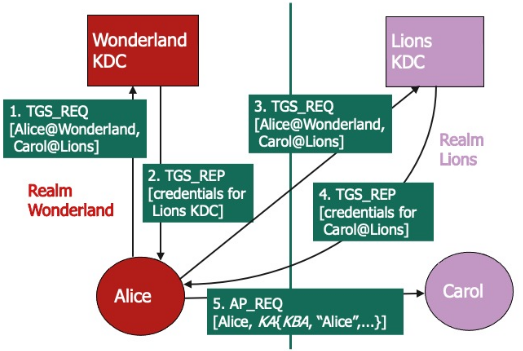
\includegraphics[width=.9\linewidth]{static/img/cysec/inter_realm_authentication.png}
\end{center}
\end{itemize}
\end{itemize}

\subsubsection*{A5. Zero-Knowledge Password Proofs}
\label{sec:orgbe549a9}
\begin{itemize}
\item DH parameters are encrypted with the user password and then transmitted
\begin{itemize}
\item resulting in a \textbf{Strong Ephemeral DH Secret} (x\textsubscript{us})
\end{itemize}
\item using this DH secret a mutual Challenge / Response is built

\begin{center}
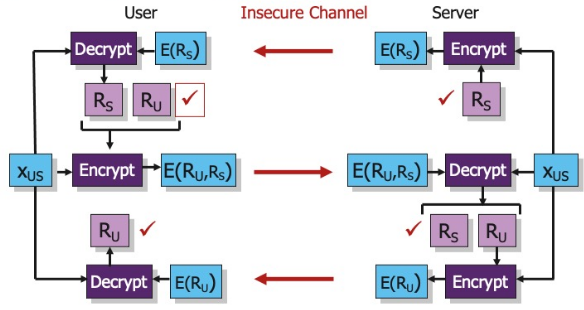
\includegraphics[width=.9\linewidth]{static/img/cysec/encrypted_key_exchange.png}
\end{center}
\end{itemize}

\subsubsection*{Summary}
\label{sec:org12e5345}
\begin{center}
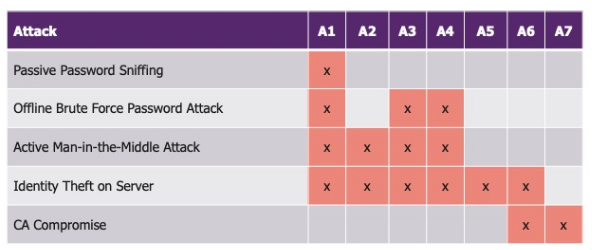
\includegraphics[width=.9\linewidth]{static/img/cysec/vulnerability_matrix.png}
\end{center}

\begin{itemize}
\item Challenge / Response based authentication schemes are the standard
\end{itemize}

\section*{Week 10 - Introduction to Ethical Hacking and Penetration Testing}
\label{sec:orgbfde033}
\subsection*{Introduction to Ethical Hacking}
\label{sec:org2108587}
\begin{itemize}
\item Attack concepts
\begin{itemize}
\item \textbf{Hacking}
\begin{itemize}
\item exploit vulnerabilities
\item security control compromise
\item produce behaviors outside of systems original intend
\end{itemize}

\item \textbf{Ethical hacking}
\begin{itemize}
\item validate, audit and report on system / software vulnerabilities
\item reporting vulnerabilities
\end{itemize}
\end{itemize}

\item Hacker types
\begin{itemize}
\item \textbf{Black Hat}
\item \textbf{Grey Hat}
\item \textbf{White Hat}
\item \textbf{Script Kiddie}
\item \textbf{Cyber Terrorist}
\item \textbf{State Sponsored} (Hacker employed by the government for offensive and defensive
\item \textbf{Hacktivism} (Hacker whoses activity is aimed at promoting a social / political cause)
\end{itemize}

\item legal aspect of pen testing
\begin{itemize}
\item pen testing contracts
\item \textbf{Statement of Work (SoW)}
\begin{itemize}
\item what is allowed, time line, which activities to be perfomred
\end{itemize}
\item \textbf{Non Disclosure agreement (NDA)}
\end{itemize}

\item penetration testing methodologies
\begin{center}
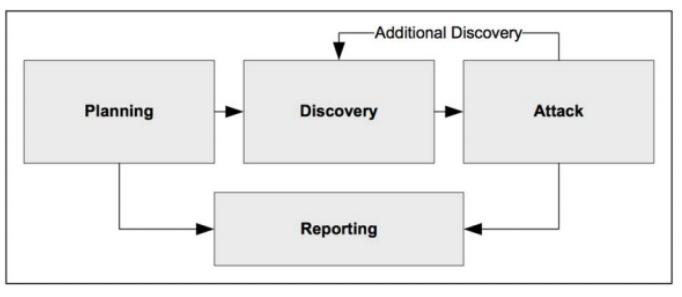
\includegraphics[width=.9\linewidth]{static/img/cysec/penetration_testing_methodologies.png}
\end{center}

\begin{center}
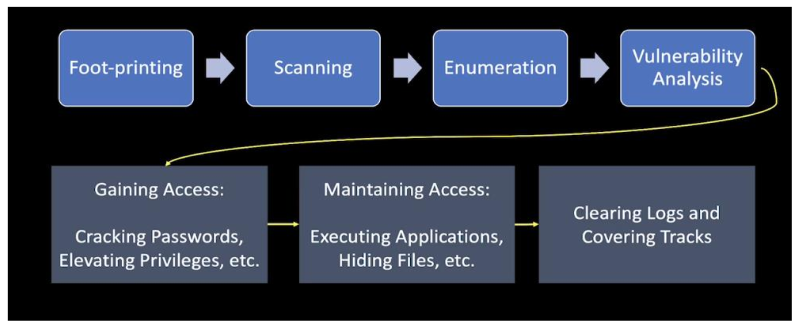
\includegraphics[width=.9\linewidth]{static/img/cysec/penetration_testing_methodologies_ec.png}
\end{center}
\end{itemize}

\subsection*{Malicious code}
\label{sec:orga5b2a11}
\begin{itemize}
\item \textbf{Zero-Day Attack}
\item source of malicious code
\begin{itemize}
\item Script kiddie
\item \textbf{Drive-by download} (you don't have to click on anything)
\item \textbf{Advanced persistent threat (ATP)} (advanced technical skills and significant financial resources
\begin{itemize}
\item often military units, intelligence agencies, affiliated with \textbf{government agencies}
\end{itemize}
\item \textbf{Viruses}
\begin{itemize}
\item two functions: \textbf{propagation} and \textbf{destruction}
\end{itemize}
\end{itemize}
\end{itemize}

\subsection*{Virus propagation techniques}
\label{sec:orgb7ae4ec}
\begin{itemize}
\item \textbf{master boot record infection}
\begin{itemize}
\item only small part of virus in MBR, MBR loads the whole virus from somewhere else (HDD)
\end{itemize}

\item \textbf{file infection}
\begin{itemize}
\item infects executable files (.com, .exe)
\end{itemize}

\item \textbf{macro infection}
\begin{itemize}
\item e.g. Office Macros
\end{itemize}

\item \textbf{service injection}
\begin{itemize}
\item inject itself into trusted runtime processes of the OS
\end{itemize}
\end{itemize}

\subsection*{Malware Technologies}
\label{sec:org9d7fc64}
\begin{itemize}
\item \textbf{Multipartite Viruses}
\begin{itemize}
\item uses more than one progpagation
\end{itemize}

\item \textbf{Stealth Viruses}
\begin{itemize}
\item hide themselves and fool antivirus
\end{itemize}

\item \textbf{Polymorphic Viruses}
\begin{itemize}
\item modify their own code as they travel from system to system
\end{itemize}

\item \textbf{Encrypted Viruses}
\begin{itemize}
\item use cryptographic techniques to avoid detection
\item short segment \textbf{virus decryption routine}
\end{itemize}

\item \textbf{Logic Bomb}
\begin{itemize}
\item infect system and lie dormant until they are trigger by a condition
\end{itemize}

\item \textbf{Trojan Horses}
\begin{itemize}
\item appears kind but carries malicious \textbf{behind-the-scenes payload}
\end{itemize}

\item \textbf{Keystroke logging}
\begin{itemize}
\item logging the keys struck on a keyboard (HW or SW)
\end{itemize}

\item \textbf{Ransomware}
\begin{itemize}
\item infect target and encrypt files; key only known by the creator
\end{itemize}

\item \textbf{Worms}
\begin{itemize}
\item propagate themselves \textbf{without requiring any human intervention}
\item e.g \textbf{Stuxnet}
\end{itemize}

\item \textbf{Spyware}
\begin{itemize}
\item monitors your action and transmits details to remote
\end{itemize}

\item \textbf{Adware}
\begin{itemize}
\item display advertisements
\end{itemize}
\end{itemize}

\subsection*{Antivirus}
\label{sec:org6ef265d}
\begin{itemize}
\item software to prevent, detect and remove malware
\item not only from viruses
\item Antivirus detection
\begin{itemize}
\item \textbf{signature based}
\item \textbf{heuristic based} (analyze behavior of software)
\item \textbf{data integrity} (sudden changes in executable file may be an sign of malware, except for updates)
\end{itemize}
\end{itemize}

\subsection*{Applications Attack}
\label{sec:org17d50bb}
\begin{itemize}
\item \textbf{Buffer Overflows}
\begin{itemize}
\item input to large for buffer => overflow
\end{itemize}

\item \textbf{Time of Check to Time of Use (TOC/TOU)}
\begin{itemize}
\item timing vulnerability; program check access permission to far
\end{itemize}

\item \textbf{Back Doors}
\begin{itemize}
\item undocumented command sequences to bypass normal access restrictions
\end{itemize}

\item \textbf{Escalation of Privileged}
\begin{itemize}
\item expand access from normal user to more administrative access
\end{itemize}

\item \textbf{Rootkits}
\begin{itemize}
\item exploit known vulnerabilities in OS and provide the hacker the possibility to increase his access to the root level
\end{itemize}
\end{itemize}

\subsection*{Web Application Attack}
\label{sec:org739b971}
\begin{itemize}
\item \textbf{Cross-Site Scripting (XSS)}
\begin{itemize}
\item embed custom JS in to the website
\end{itemize}

\item \textbf{Cross-Site Request Forgery (XSRF or CSRF)}
\begin{itemize}
\item embed code in one website that sends a command to a second website
\end{itemize}

\item \textbf{Dynamic Web Applications}
\begin{itemize}
\item possible way from webserver (DMZ) to gain access to DB server (LAN)
\item firewall rules has to be corret
\end{itemize}

\item \textbf{SQL Injection}
\begin{itemize}
\item inject malicious SQL
\end{itemize}
\end{itemize}

\subsection*{Network security}
\label{sec:org3f218c1}
\begin{itemize}
\item why hacking network devices
\begin{itemize}
\item old protocols
\item long system life cycle
\item no malware detection
\end{itemize}

\item \textbf{Attacks}
\begin{itemize}
\item \textbf{Denial-of-Service (DoS)}
\begin{itemize}
\item \textbf{System overload} and \textbf{Link overload}
\item \textbf{SYN flooding}
\item \textbf{Service request floods}
\item \textbf{Application level DoS} (usage of a vulnerability to cause a crash / hang / freeze / consume all resources)
\item \textbf{Permanent DoS} (installing compromised HW updated to destroy the HW)
\end{itemize}

\item \textbf{Botnets}
\begin{itemize}
\item bot / zombie are controlled over the C\&C (Command \& Control) from the botmaster
\item \textbf{Distributed DoS (DDoS)}
\end{itemize}

\item \textbf{Man-in-the-Middle (MITM)}
\begin{itemize}
\item active and passive
\end{itemize}

\item \textbf{Man-in-the-Browser}
\begin{itemize}
\item Browser Plugin installed; Capture form data (username / password)
\end{itemize}

\item \textbf{Eavesdropping}
\begin{itemize}
\item listen to communication traffic for the purpose of duplicating it
\item Wireshark
\end{itemize}

\item \textbf{Impersonation / Masquerading}
\begin{itemize}
\item pretending to be someone / something you are not
\item unusually authentication credentials have been stolen
\item Not the same as \textbf{Spoofing} (Spoofing uses a false identity but without proof)
\end{itemize}

\item \textbf{Replay Attacks}
\begin{itemize}
\item replay a captured (e.g with Wireshark) traffic to reestablish communication
\end{itemize}

\item \textbf{Modification Attacks}
\begin{itemize}
\item captured packets are altered and then played against a system
\end{itemize}
\end{itemize}
\end{itemize}


\subsubsection*{Session hijacking}
\label{sec:orgfceaca0}
\begin{itemize}
\item \textbf{Session IDs}
\begin{itemize}
\item used to establish a stateful connection
\item stored in cookies, passed in URL or hidden fields
\end{itemize}

\item \textbf{Session hijacking with session predicting}
\begin{itemize}
\item watch session IDs for pattern and tries to predict
\end{itemize}

\item \textbf{Session hijacking with session fixation}
\begin{itemize}
\item 
\end{itemize}

\item \textbf{Session hijacking with Cross-Site Scripting}
\begin{itemize}
\item embed JS in website sends Session ID to attacker when client established a connection
\end{itemize}

\item \textbf{Session hijacking with Cross-Site request forgery}
\begin{itemize}
\item Client establish connection to server; if user clicks on a malicious link the attacker can use the established session
\end{itemize}

\item \textbf{Session hijacking with TCP/IP hijacking}
\begin{itemize}
\item Normal TCP 3-way handshake
\item attacker responds quicker to the SYN/ACK then the regular client
\end{itemize}
\end{itemize}

\section*{Week 11 - Federation}
\label{sec:org3542ac9}
\subsection*{Federations}
\label{sec:org212df2e}
\begin{itemize}
\item \textbf{Federation Identity Management}
\begin{itemize}
\item agreements, standards and technologies to make \textbf{identity} and \textbf{entitlements portable} across autonomous identity domains
\end{itemize}

\item \textbf{Federated Identity}
\begin{itemize}
\item is the means of linking a person's electronic identity and attributes, stored across multiple distinct identity management systems
\end{itemize}

\item \textbf{Federation}
\begin{itemize}
\item a set of organizations agreeing on a common set of rules and standard
\item[{goal}] cooperate in inter-organizational authentication, authorization and accounting
\end{itemize}
\end{itemize}


\begin{itemize}
\item \textbf{Identity Provider (IdP)}
\begin{itemize}
\item perform authentication
\end{itemize}

\item \textbf{Service Provider (SP)}
\begin{itemize}
\item offers service and performs authorization
\end{itemize}
\end{itemize}

\subsection*{Shibboleth}
\label{sec:org7bcaa9c}
\begin{itemize}
\item protocol to implement
\end{itemize}


\begin{enumerate}
\item Phase - User connect to resource and is redirected
\begin{itemize}
\item If already a valid Shibboleth session is available, you get access to \textbf{the resource}
\item if no session is active you get redirected to the \textbf{Discovery Service}. This sends you a page with all \textbf{Home Organizations}
\end{itemize}

\item Authentication Request
\begin{itemize}
\item choose \textbf{Home Organization} and the Discovery Service responses with a redirect to the \textbf{session initiator} of the resource
\item the session initiator creates an authentication request for the Home Organization and sends it through the browser to the Home Organization
\item Home Organization evaluates the authentication request and present a login page
\end{itemize}

\item Authentication and Access
\begin{itemize}
\item user provides his credentials; credentials are checked and an \textbf{assertion} including the users attributes is created
\item the assertion is submitted through the browser back to the resource. Resource can perform authorization checks
\end{itemize}
\end{enumerate}


\begin{center}
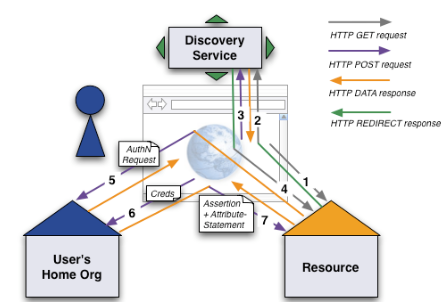
\includegraphics[width=.9\linewidth]{static/img/cysec/shibboleth.png}
\end{center}

\subsection*{XML Security and SAML}
\label{sec:org82b3382}
\begin{itemize}
\item \textbf{Secure Assertion Markup Lnaguage (SAM)}
\begin{itemize}
\item XML-encoded assertions about authentication, attributes and authorization
\item Allows single sing-on solution for web services
\end{itemize}
\end{itemize}

\subsection*{OAuth 2 Authorization Framework}
\label{sec:orgf37c162}
\begin{description}
\item[{goal}] app can access you data at some service but without knowing your password

\item Roles
\begin{itemize}
\item \textbf{Client}
\begin{itemize}
\item making requests on behalf of the resource owner and with its authorization
\end{itemize}

\item \textbf{Resource Owner}
\begin{itemize}
\item entity capable of granting access to protected resources
\end{itemize}

\item \textbf{Resource Server}
\begin{itemize}
\item server hosting the protected resources
\end{itemize}

\item \textbf{Authorization Server}
\begin{itemize}
\item issuing access tokens to the client
\end{itemize}
\end{itemize}
\end{description}

\begin{center}
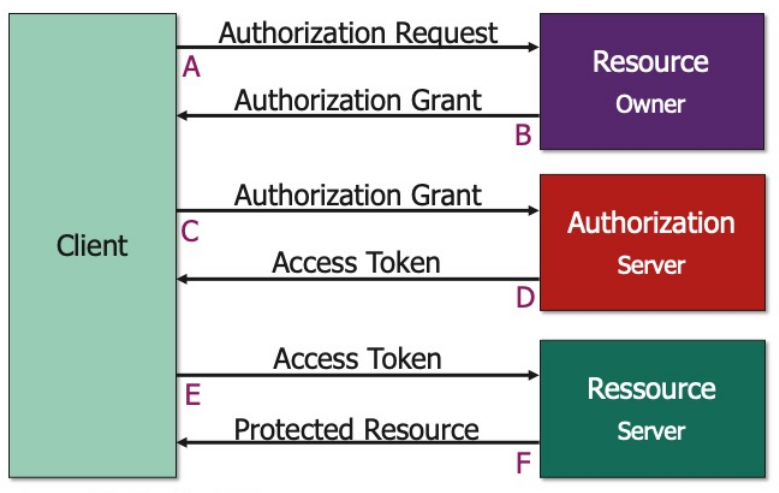
\includegraphics[width=.9\linewidth]{static/img/cysec/oauth2_protocol_flow.png}
\end{center}

\subsection*{OpenID Connect Authentication Layer}
\label{sec:org550f062}
\begin{itemize}
\item solves the problem of
\begin{itemize}
\item one ID per site
\item managing passwords per site
\item layer on top of OAuth 2.0
\end{itemize}

\item decentralized mechanism for \textbf{single sign-on}
\begin{itemize}
\item access different sites using the same identity
\item website never sees your password
\end{itemize}

\item used by Google, Microsoft, PayPal, \ldots{}
\item access token contains:
\begin{itemize}
\item user ID
\item approved scopes
\item expiration
\end{itemize}
\item[{example}] \textbf{SwissID}

\item \textbf{Relying Party (RP)} same as Service Provider (PostFinance)
\item \textbf{OpenID Provider (OP)} same as Identity Provider (SwissID)

\item RP (OAuth Client) requests a signed ID Token authenticating User (Resource Owner) from OP (Authorization/Resource Server)
\end{itemize}

\section*{Week 12 - Email Security}
\label{sec:orgda14bcb}
\subsection*{S/MIME}
\label{sec:orgf9e4e35}
\textbf{Multipurpose Internet Mail Extension (MIME)}

\textbf{S/MIME} type 1: multipart entity with subtype \textbf{multipart/signed}. contains two bodies:
\begin{enumerate}
\item content to be signed (regular mime)
\item digital signature over content part, with subtype \textbf{pkcs7-signature}
\end{enumerate}
signature also possible over multipart/mixed

\textbf{S/MIME} type 2: MIME content carried withing an \textbf{PKCS\#7 Signed Data Object (*smime-type=signed-data;})
\begin{itemize}
\item pro: MIME content is not prone to changes during transfer
\item contra: in order to read the mail, the receiver's mail client must support S/MIME
\end{itemize}

\textbf{S/MIME - Encrypted Message Format}:
\begin{itemize}
\item Content-Type: \textbf{application/pkcs7-mime;} \textbf{smime-type=envelped-data;}
\item to send an encrypted message to multiple recipients encrypt content symmetric and then encrypt key with each others public key
\end{itemize}

\textbf{PKCS \#7 - Public Key Cryptography Standard}:
contains a \textbf{SignedData} block
\begin{itemize}
\item version, digestAlgorithms, contentInfo, certificates, crls, signerInfos (several signers possible)
\end{itemize}
SignedData contains \textbf{SingerInfo} block
\begin{itemize}
\item version, issuerAndSerialNumber, digestAlgorithm, authenticatedAttributes, digestEncryptionAlgorithm, encryptedDigest (signature), unauthenticatedAttributes
\end{itemize}

Storage of keys
\begin{itemize}
\item \textbf{Signature Key}
\begin{itemize}
\item equivalent to a person's digital identity
\item must not be more than a single copy
\item best store on smart cards
\end{itemize}

\item \textbf{Encryption Key}
\begin{itemize}
\item backup copy protects against information loss
\item in a corporate environment deputy (stv.) should be able to access the encrypted emails if owner is absent (vacation, accident, sickness, death)
\end{itemize}
\end{itemize}

\subsection*{SPAM}
\label{sec:orgf3e9702}
\textbf{Sender Policy Framework (SPF)}: a SPF record indicate which servers are allowed to send e-mail on behalf of the domain

\textbf{Domain Keys Identified Mail (DKIM)}: SMTP server hash content and encrypt it with private key; receiver can decrypt it with public key (queried over DNS) and compare hash (basically a signature)

\textbf{Black Listing}: blocks mails from IPs

\textbf{Grey Listing}: refuse deilvery of mail with unknown triplet; Greylist Triplet:
\begin{itemize}
\item IP address
\item envelope sender address
\item envelope recipient address
\end{itemize}

\section*{Week 13 - Detect and Respond}
\label{sec:org02d350a}
\textbf{Technical vulnerability management} is a security practice to proactively mitigate / prevent exploitation of vulnerabilities. The process involves the:
\begin{enumerate}
\item identification
\item classification
\item remediation (en für Sanierung / Behebung)
\item mitigation of vulnerabilities
\end{enumerate}

\begin{center}
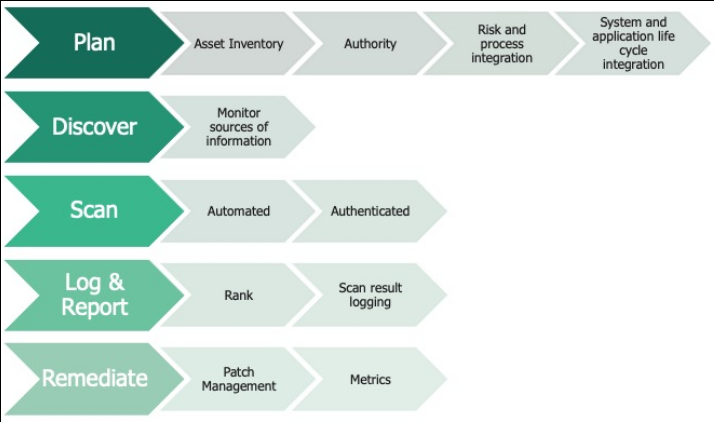
\includegraphics[width=.9\linewidth]{static/img/cysec/vulnerability_management_steps.png}
\end{center}

\textbf{Plan} is the process of Risk and process integration, integrating with asset inventory, establishment of a clear authority to review vulnerabilities and system and application life cycle integration

\textbf{Discover} step involves monitoring sources of information about known vulnerabilities (e.g CVSS, NIST, CERT, \ldots{})

\textbf{Scan} regulary software, systems and networks for vulnerabilites and proactively address those. But scanning can cause disruptions and huge amount of data

\textbf{Log \& Report} after scan the result should be logged so that a person can verify the activity. Each vulnerability should be ranked with skill to fix, availability to attackers, privilege gained and risk and impact if exploitation is successful

\textbf{Remediate} perform patches. Ideally every discovered vulnerability should be patched immediately. But availability and the impact of a patch needs to be taken in account. Special care if multiple automated patching systems are used


\textbf{Security Event} an occurrence consider by an organization to have potential security risk. A \textbf{Security incident} is an occurrence that actually or potentially jeopardizes the confidentiality, integrity or availability (CIA).

\textbf{Security Event Management (SEM)} should help to identify threats that may lead to an security incident, maintain integrity, conditionality and availability. For this the logs has to go through the following steps: 
\begin{enumerate}
\item \textbf{Normalization} - data in common format
\item \textbf{Filtering} - assigning priorities and set a large amount aside
\item \textbf{Aggregation} - group multiples events in one bigger (where useful)
\end{enumerate}
To generate alerts you can perform \textbf{Pattern matching} on logs, detect a scan (\textbf{Scan detection}), to many occurrence of a security event (\textbf{Threshold detection}) or detect correlation between multiple events which indicate a security incident (\textbf{Event correlation}).

\textbf{Thread Intelligence} is the knowledge established as a result of analyzing information about potential / current attacks.

\textbf{Cyber Attack Kill Chain} consist of Reconnaissance, Weaponization, Delivery, Exploit, install action, C\&C, Action

\textbf{Security Incident Management Process} is a process of:
\begin{itemize}
\item \textbf{Preparation}: define what is a incident, answer WHO-WHEN-WHAT, response and reporting procedure, guidelines for communication
\item \textbf{Detection \& Analysis}: detected then magnitude (e.g. number of affected devices), severity (what it the sensitivity of the data), urgency (active problem, threat or an event-in-progress). The analysis needs to determine whether immediate actions is needed.
\item \textbf{Containment, Eradication \& Recovery}: most incidents require some sort of containment. Strategies for dealing with various types of incident must be planned well in advance (system isolation, disable system-level accounts, terminate active session, \ldots{}). During recovery restore systems to normal operation and harden systems where applicable
\item \textbf{Post-Incident Activity}: follow-up report and lessons learned
\end{itemize}


\textbf{Phases of Digital Forensics Process}:
\begin{center}
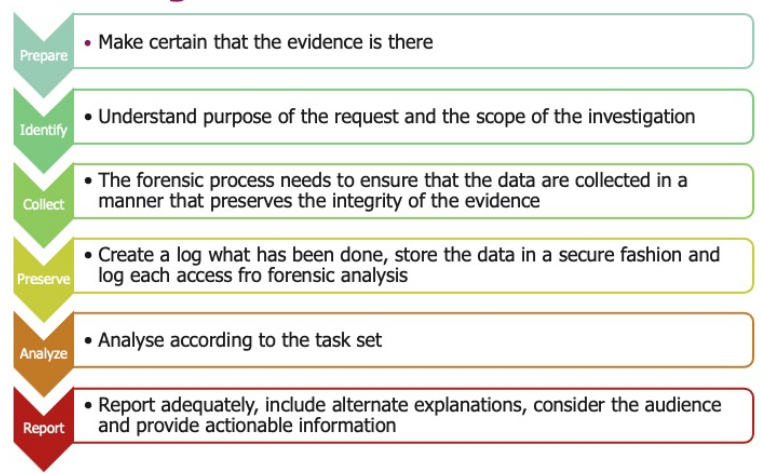
\includegraphics[width=.9\linewidth]{static/img/cysec/phases_of_digital_forensics.png}
\end{center}

Threat and incident management best practice
\begin{enumerate}
\item Cybersecurity resilience (en für Belastbarkeit): Technical vulnerability management, Security event logging, Security event management, Threat intelligence, Cyber attack protection
\item Security incident management: Security incident management framework, Security incident management process, Emergency fixes, forensic investigation
\end{enumerate}

\section*{Week 14 - Web Application Security}
\label{sec:org1aa9204}
\textbf{User Credentials}: The simplest attack to hack a system is to attack the user credentials using e.g. \textbf{Spear Phishing}, \textbf{Password breached}

\begin{itemize}
\item \textbf{A1: Injection}: Injection flasws such as SQL, OS, and LDAP injections (untrusted data is sent to an interpreter as a part of a command.
\item \textbf{A2: Broken Authentication}: authentication / session management implemented incorrectly
\item \textbf{A3: Sensitive Data Exposure}: APIs often don't protect sensitive data properly (financial, PII, PHI)
\item \textbf{A4: XML external Entities (XXE)}: older / poorly configured XML processors evaluated external entity references
\item \textbf{A5: Broke Access Control}: what the users is allowed to to is often not properly enforced
\item \textbf{A6: Security Misconfiguration}: most commonly seen issue, insecure default configuration
\item \textbf{A7: Cross-Site Scripting (XSS)}: occurs when site include untrusted data in website without proper validation / escaping
\item \textbf{A8: Insecure Deserialization}: untrusted data deserialization can leads to remote code execution (do not trust data from user)
\item \textbf{A9: Using Components with known vulnerabilities}: check regularly for known bugs in your library
\item \textbf{A10: Insufficient Logging \& Monitoring}: allows attack to maintain persistence, tamper, extract or destroy data. Most breaches are over 200 days old until detected, typically detected by external parties rather than internal processes
\end{itemize}
\section*{End}
\label{sec:org440fa88}
\end{multicols}
\end{document}